\section{ByteTransformer}

\begin{frame}{Problem to Solve I: Oppornunities}
    \footnotesize{
        \hl{To achieve low latency} for an inference system that processes data online, what performance space can be leveraged?
        \begin{enumerate}
            \item the transformer block is memory bounded.
            \item prompts have variable-length, padding them into a fixed length requires redundant computations.
        \end{enumerate}
    }
\end{frame}

\begin{frame}{Problem to Solve II: Variable-length challenges MHA}
        \begin{figure}[ht]
            \begin{minipage}[b]{0.5\linewidth}
                \centering
                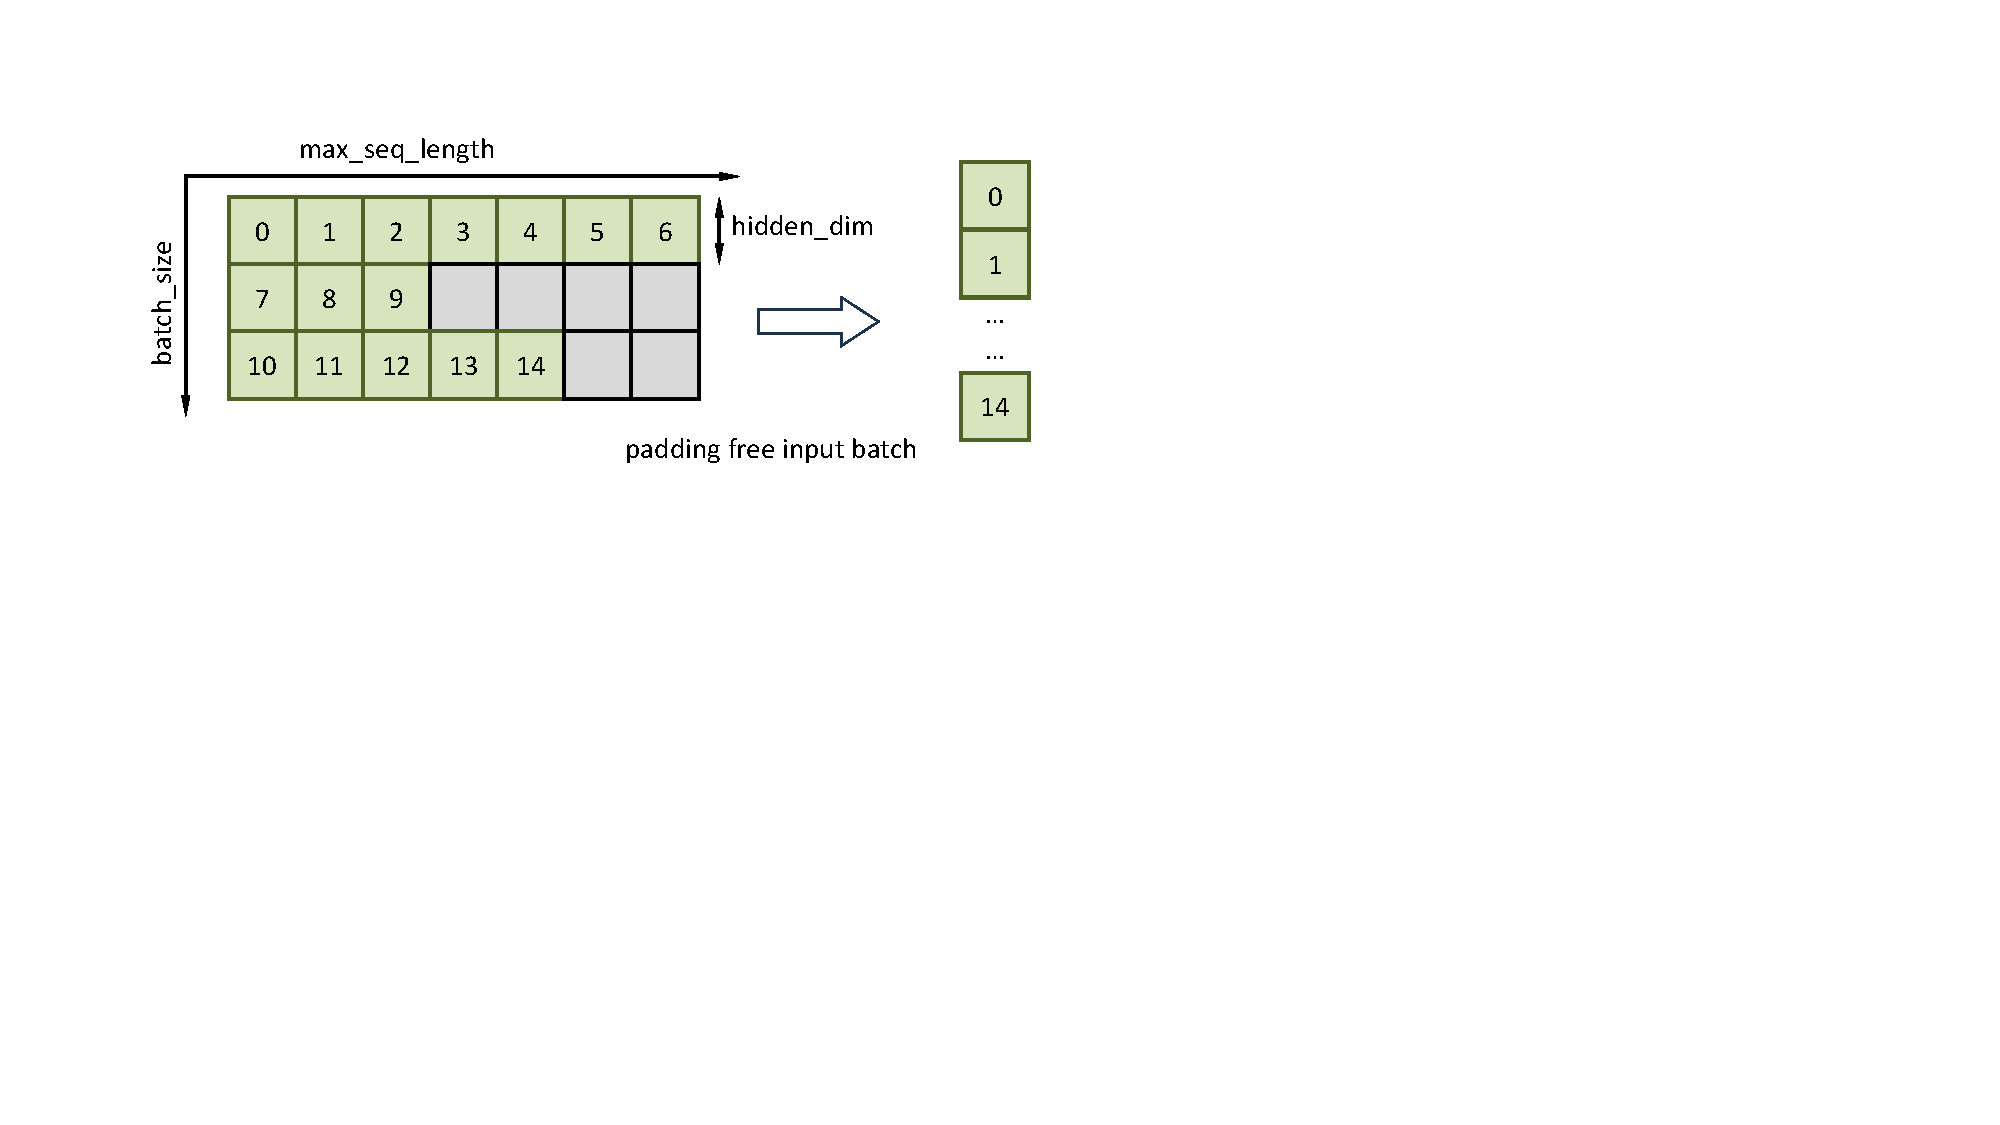
\includegraphics[width=\textwidth]{./images/bytetransformer-padding-free-input-batch.pdf}
                \footnotesize{\caption{Padding free input batch.}}
            \end{minipage}
            \hspace{0.5cm}
            \begin{minipage}[b]{0.3\linewidth}
                \centering
                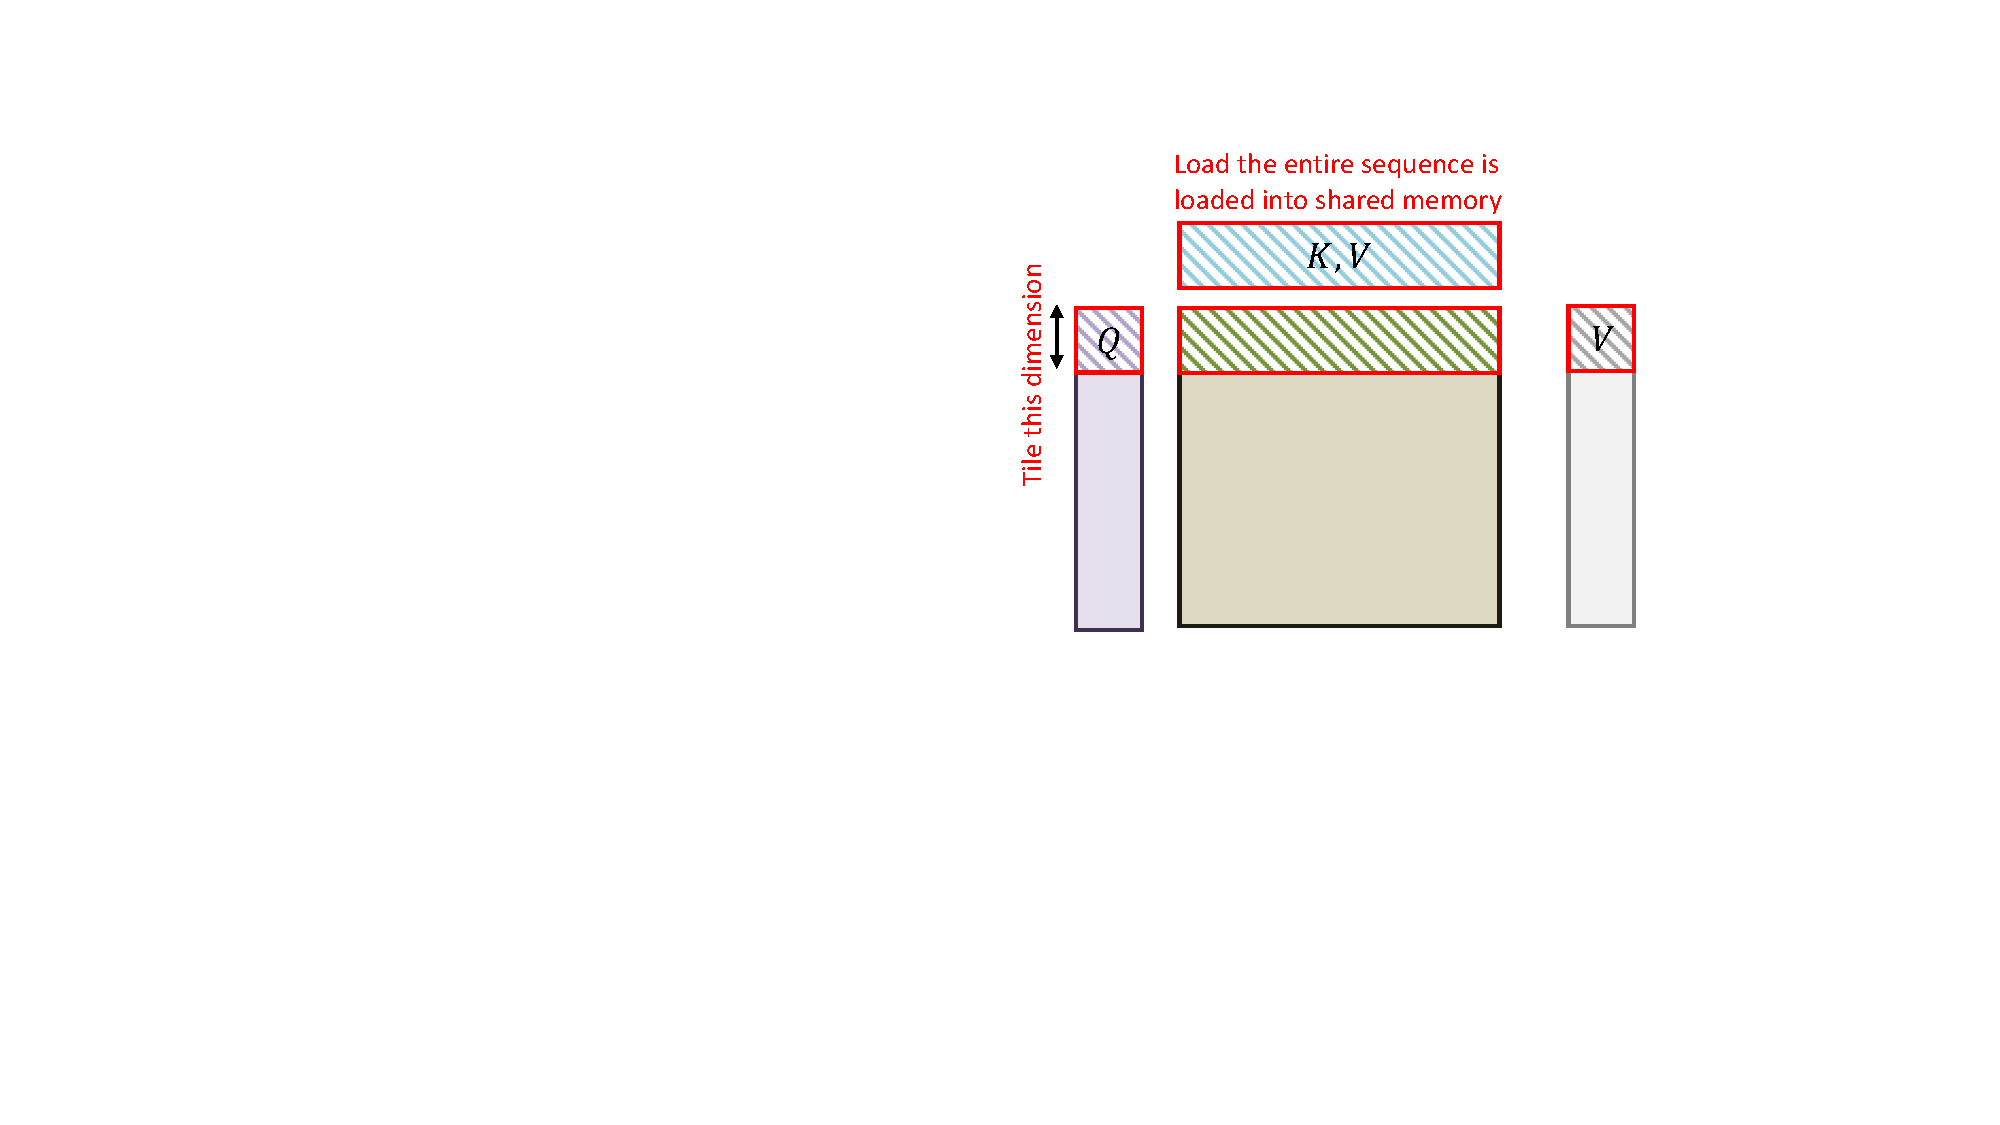
\includegraphics[width=\textwidth]{images/MHA-variable-seq-length.pdf}
                \footnotesize{\caption{MHA with variable-length sequence batch.}}
            \end{minipage}
        \end{figure}
    \footnotesize{
        \textbf{Challenges}: The computation of MHA is coupled with the sequence length dimension.
        \begin{itemize}
            \item To make it efficiently computed, batched GEMM is used. However, batched GEMM requires requires matrix multiplications to have a same shape.
        \end{itemize}
    }
\end{frame}

\begin{frame}{Solution: Padding Free + Kernel Fusion}
    \begin{figure}
        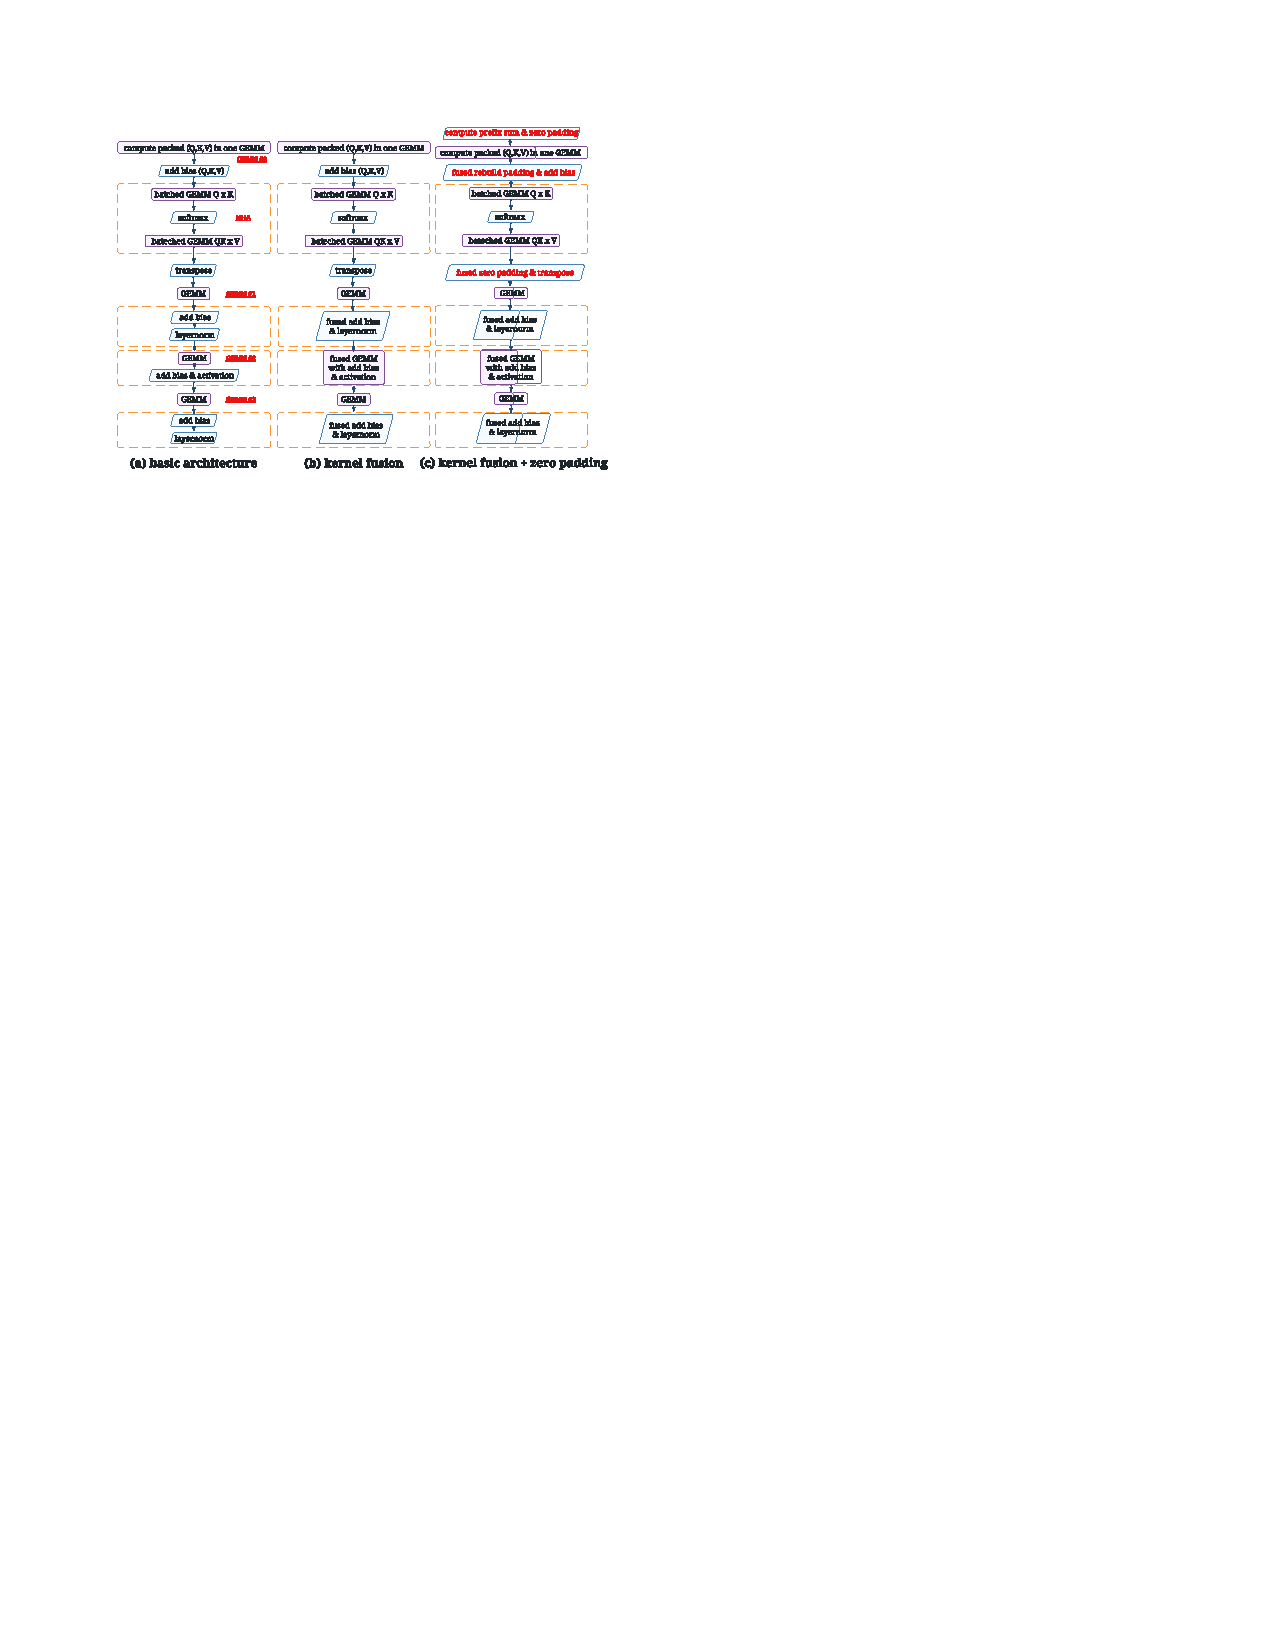
\includegraphics[width=1\linewidth]{./images/bytetransformer_overview.pdf}
        \caption{Compare ByteTransformer with other kernel fusion methods.}
    \end{figure}
\end{frame}

\begin{frame}{Solution: Padding and Padding Rebuild for MHA}
\begin{columns}[c]
    \begin{column}{.5\textwidth}
    \begin{figure}
        \centering
        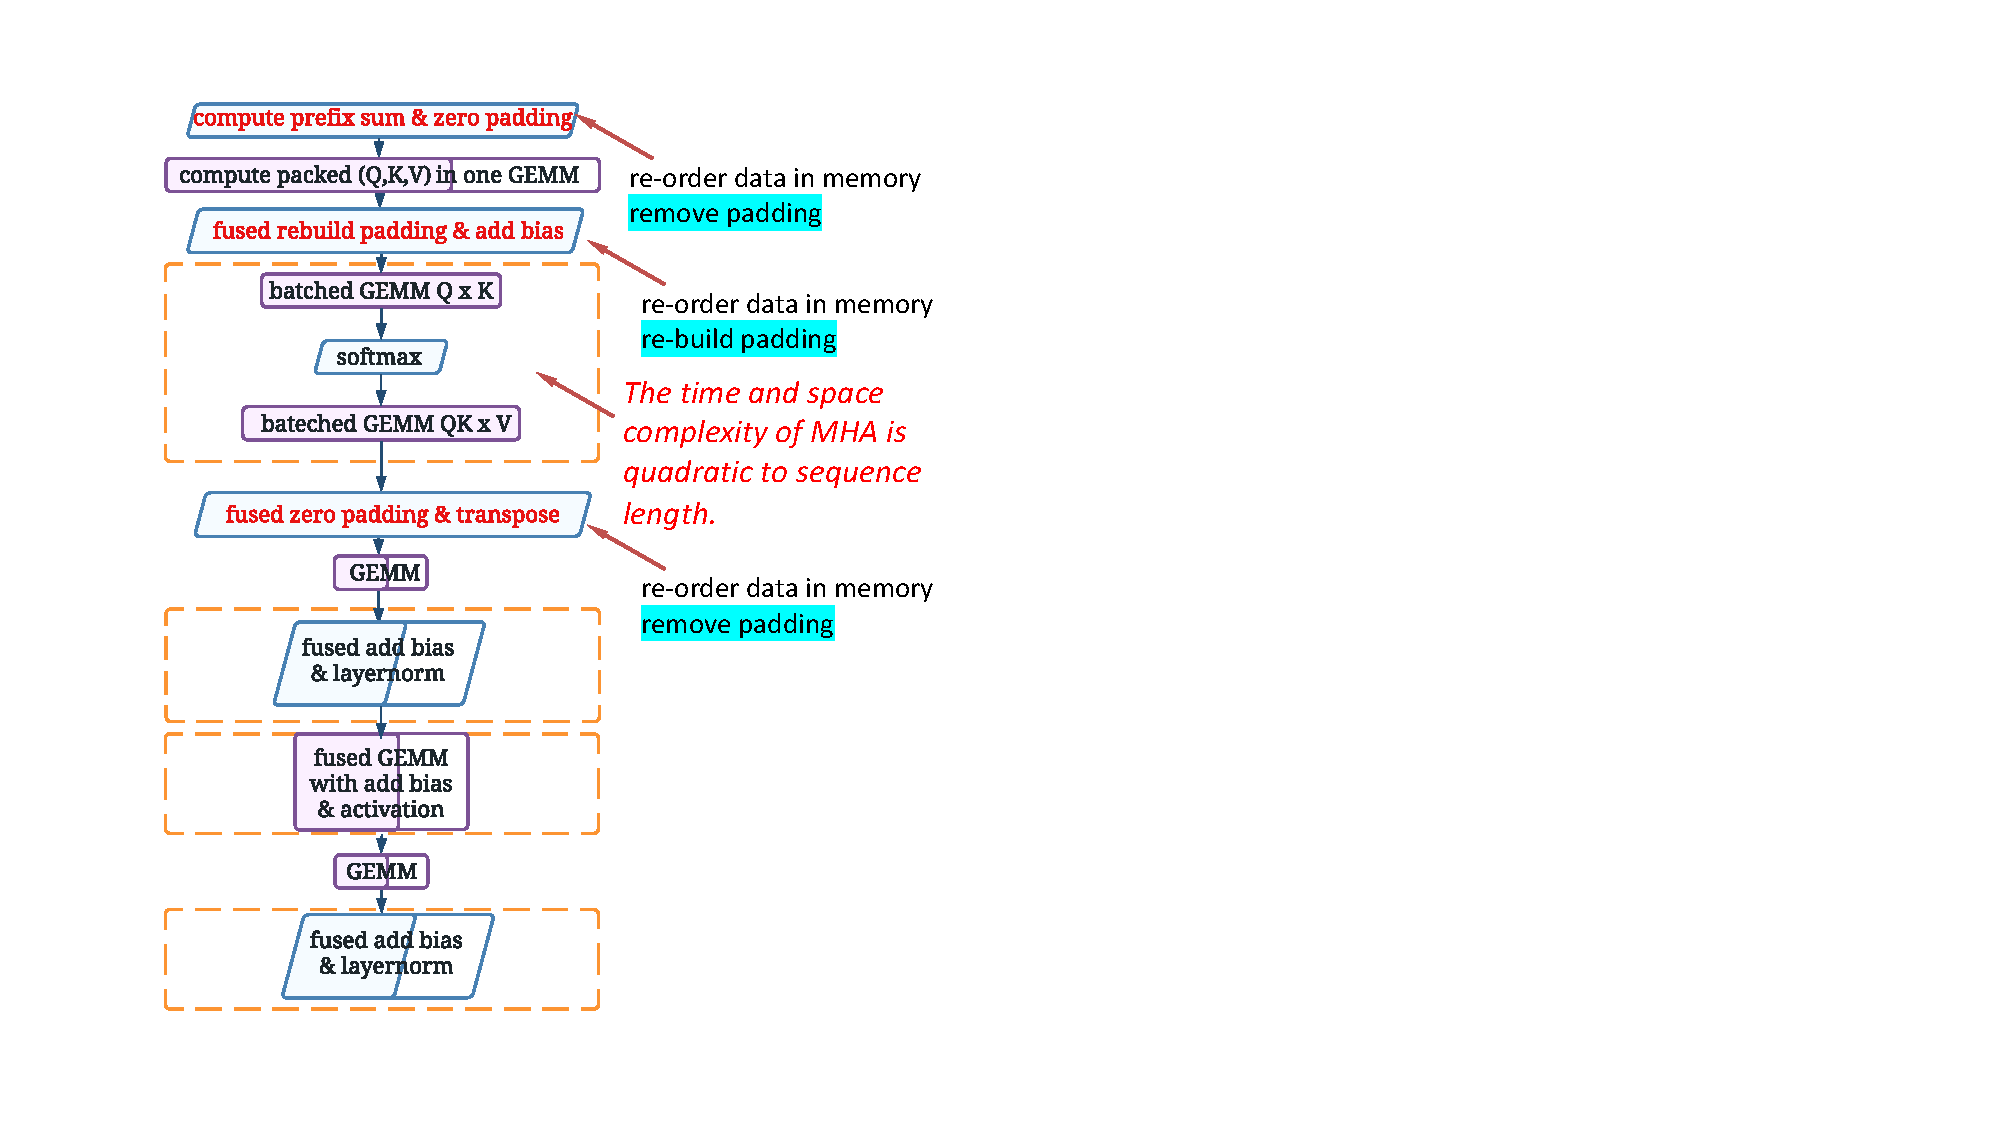
\includegraphics[width=1.\textwidth]{./images/byte-transformer-overview2.pdf}
        \caption{Overview of the ByteTransformer.}
    \end{figure}      
    \end{column}

    \begin{column}{.5\textwidth}
        % \scriptsize{
        %     \begin{itemize}
        %         \item Before MHA, insert a specially implemented kernel to re-order the input sequence batch to make it padding-free.
        %         \item When entering MHA, re-build the sequence batch again which is padded again.
        %         \item After leaving the MHA, or-order the input sequence batch to make it padding-free again.
        %     \end{itemize}
        % }
        \begin{figure}
            \centering
            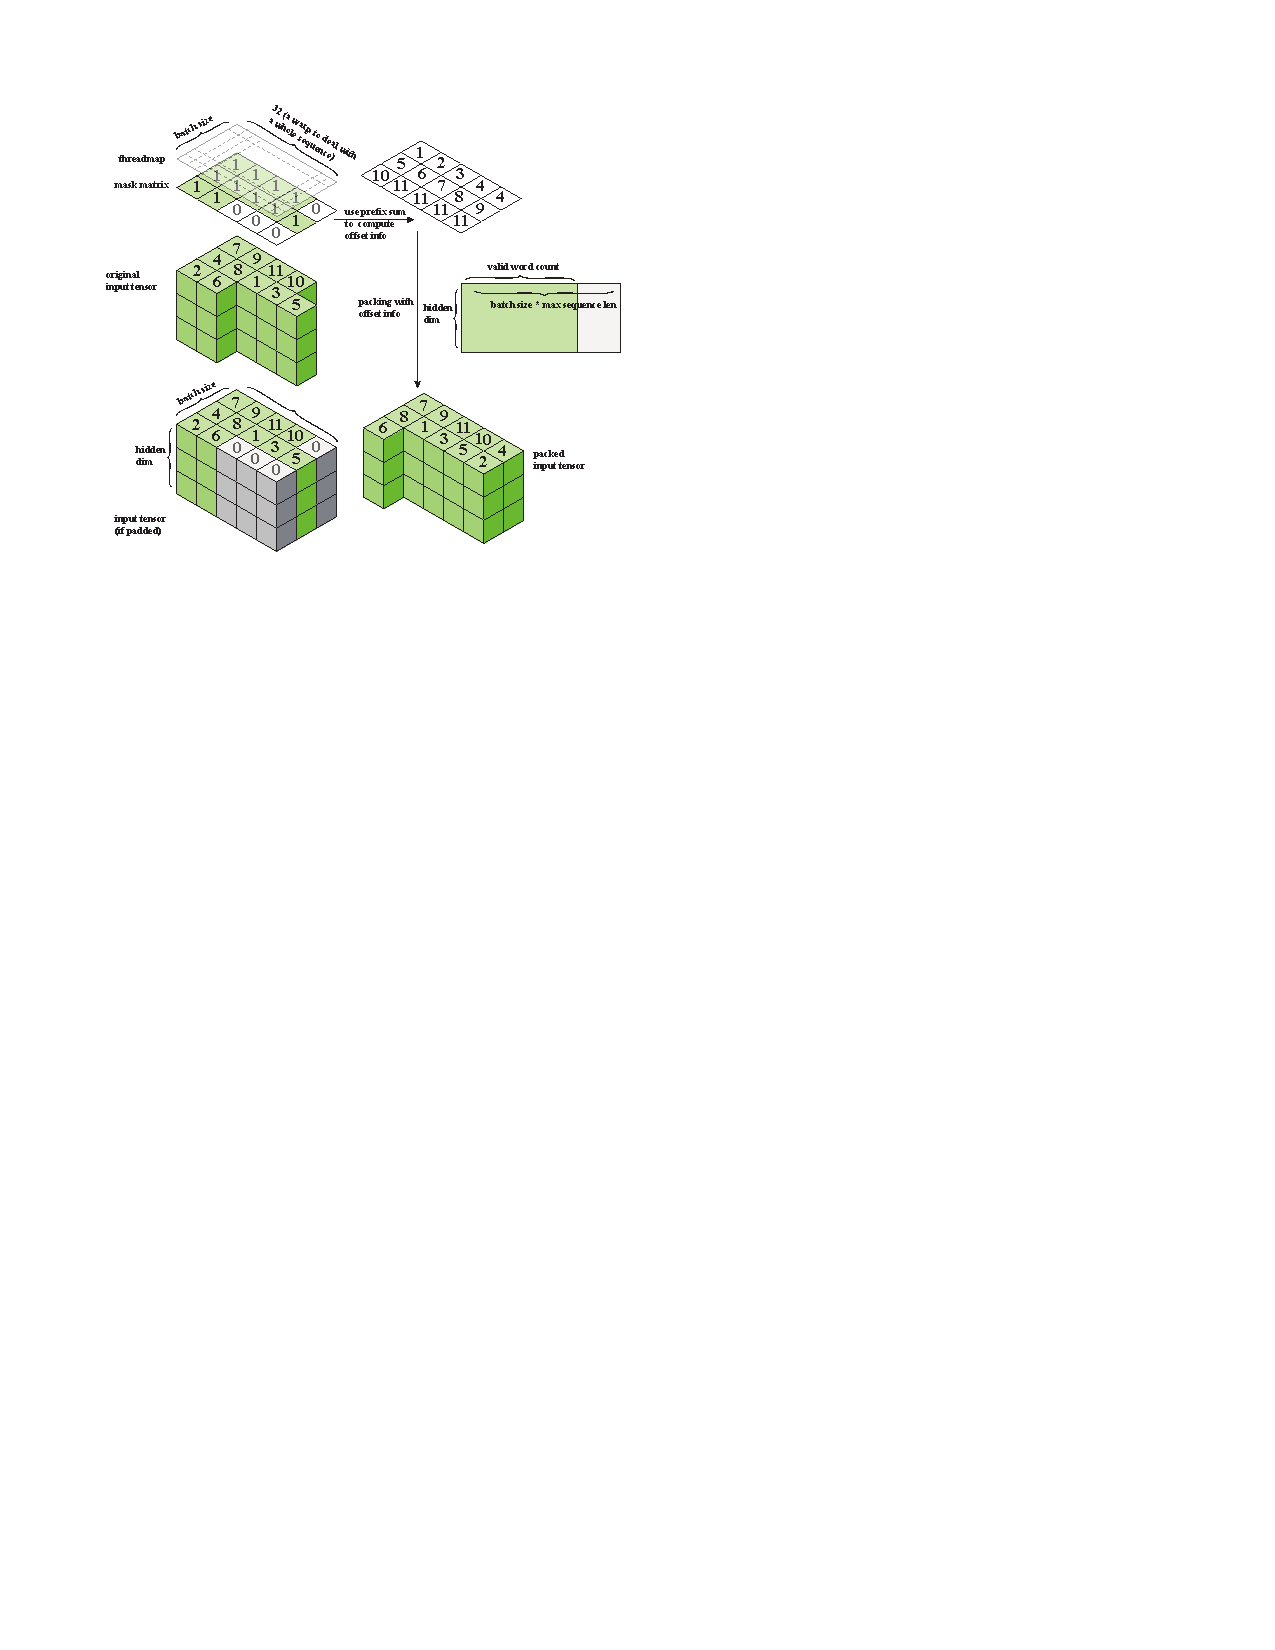
\includegraphics[width=1.\textwidth]{./images/zero-padding-algorithm.pdf}
            \caption{The padding-free operation.}
        \end{figure}  
    \end{column}
\end{columns}
\end{frame}

\begin{frame}{Optimized MHA Kernel: Short Sequences ($\le$384 tokens)}
    \begin{figure}
        \centering
        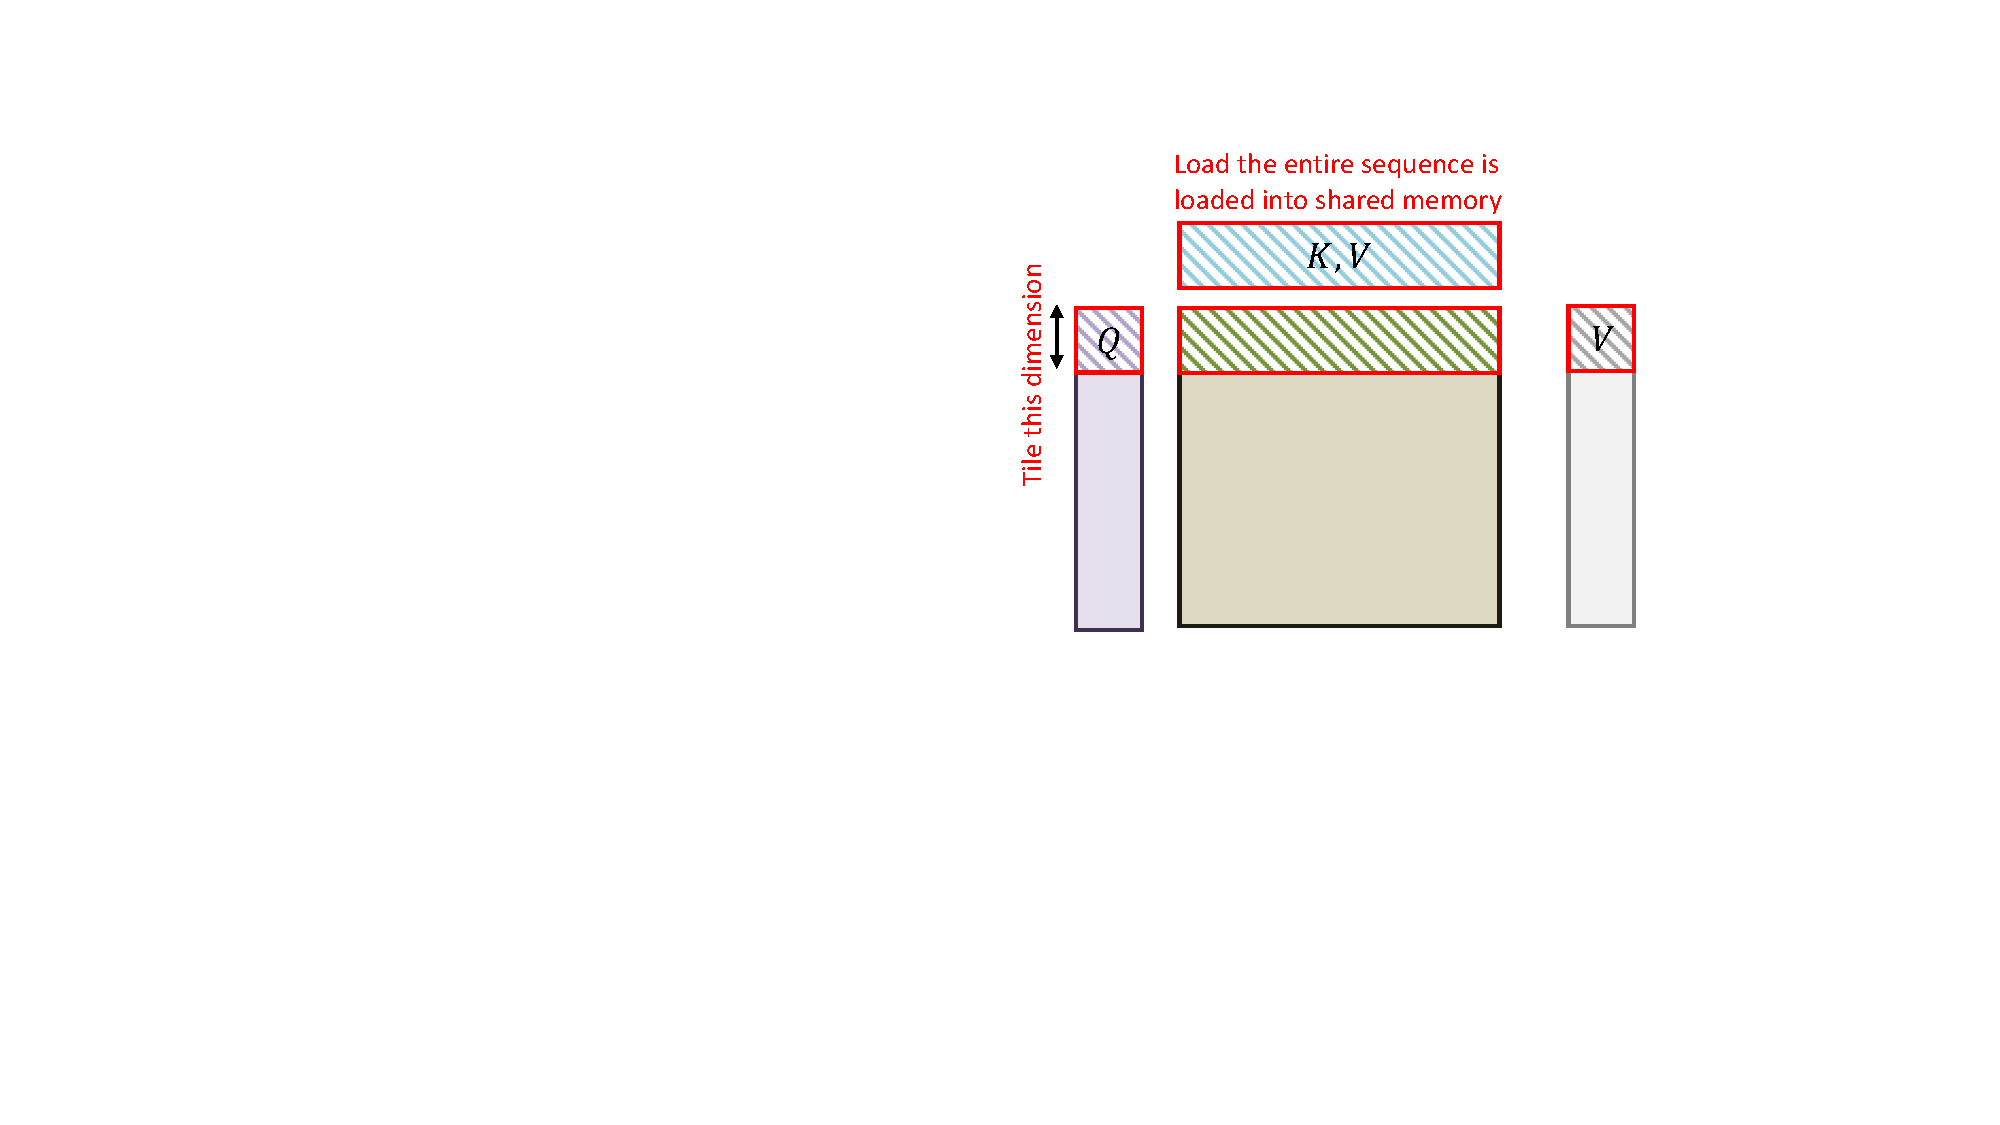
\includegraphics[width=.4\textwidth]{./images/MHA-variable-seq-length.pdf}
        \caption{Workload assigned to a CTA.}
    \end{figure}

    \begin{itemize}
        \item Tile $Q$ length, and move the entire $K$, $V$ sequence into shared memory.
        \item Keep the entire MHA computation on shared memory.
    \end{itemize}
\end{frame}

\begin{frame}{Optimized MHA Kernel: long Sequences (>384 tokens)}
    \begin{columns}[c]
        \begin{column}{.5\textwidth}
        \begin{figure}
            \centering
            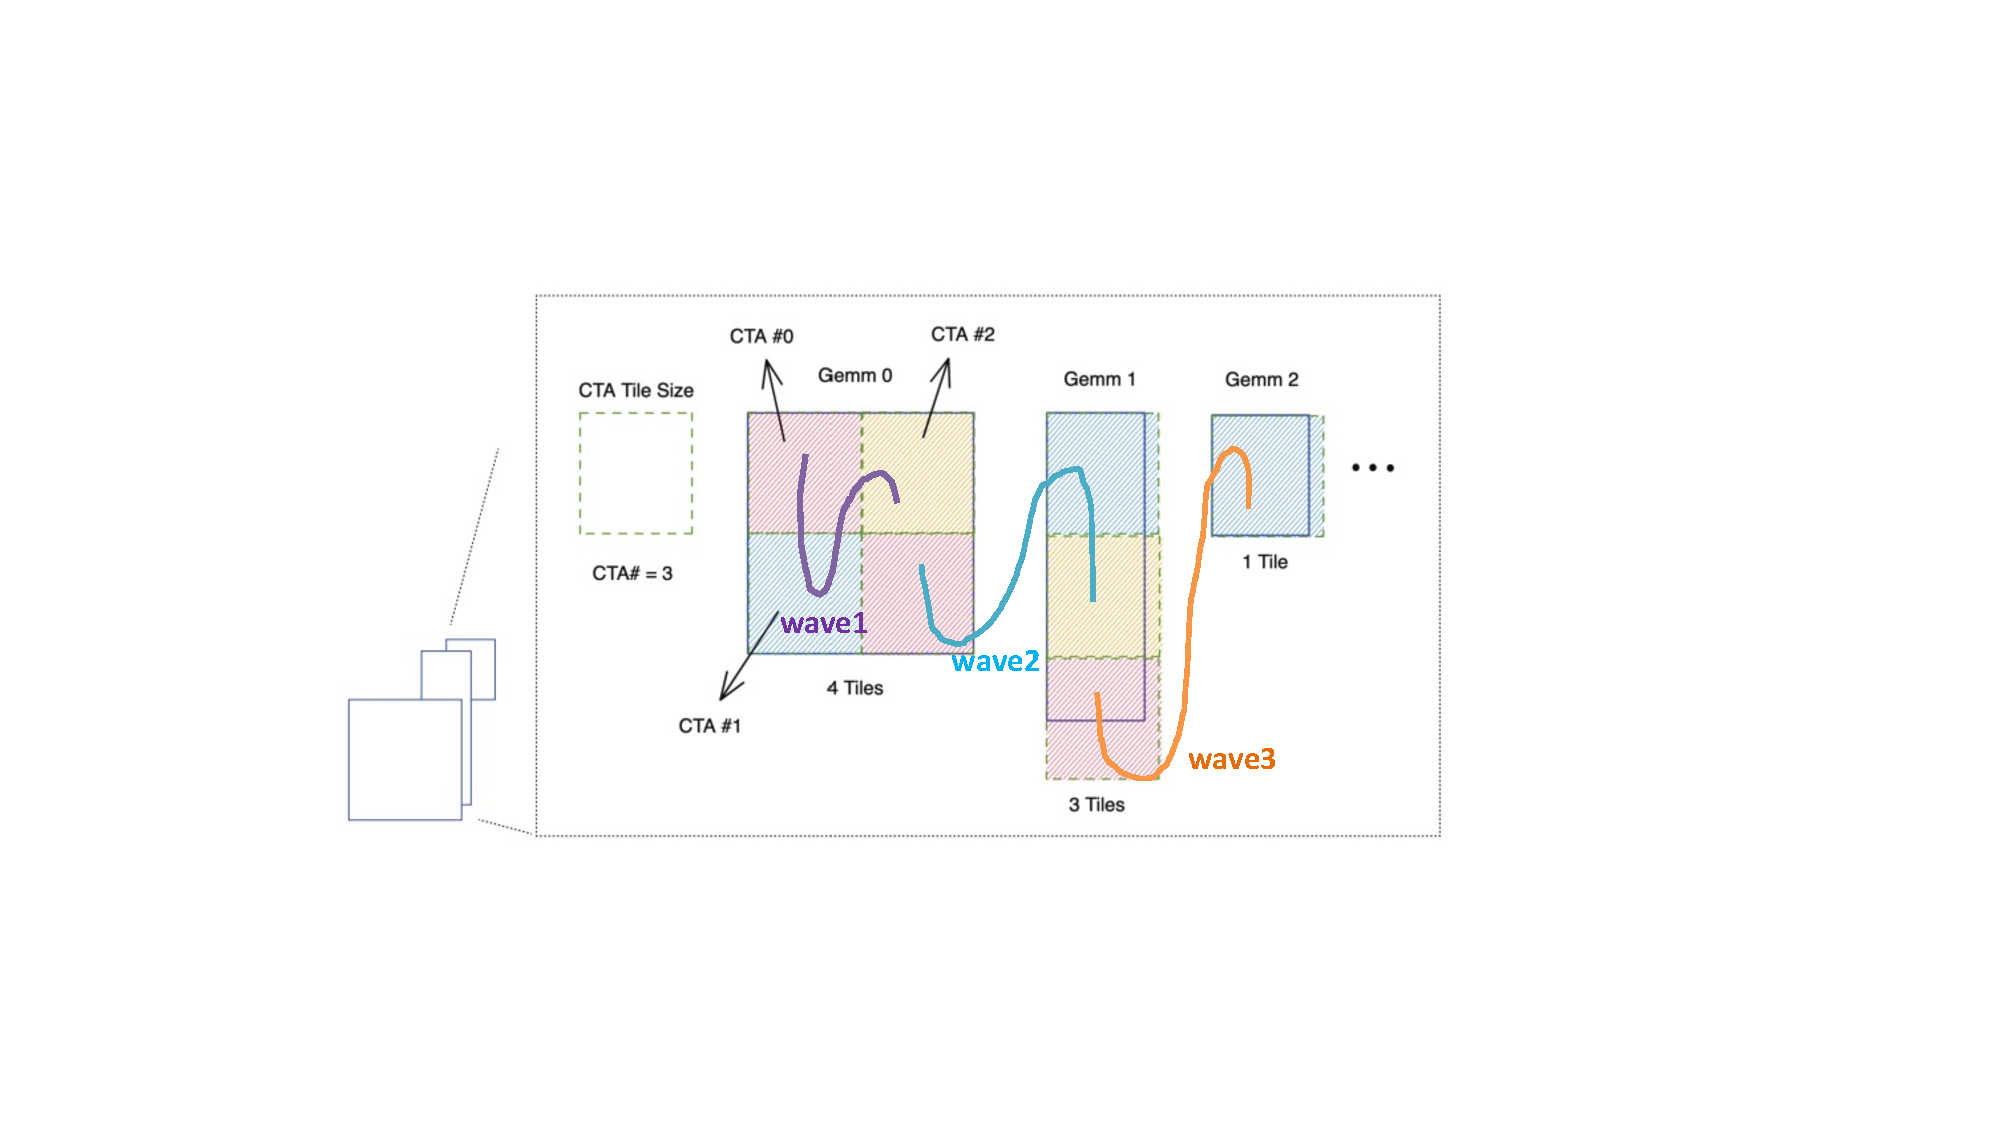
\includegraphics[width=1.\textwidth]{./images/grouped-gemm.pdf}
            \caption{The grouped GEMM operation.}
        \end{figure}      
        \end{column}
    
        \begin{column}{.5\textwidth}
            \begin{figure}
                \centering
                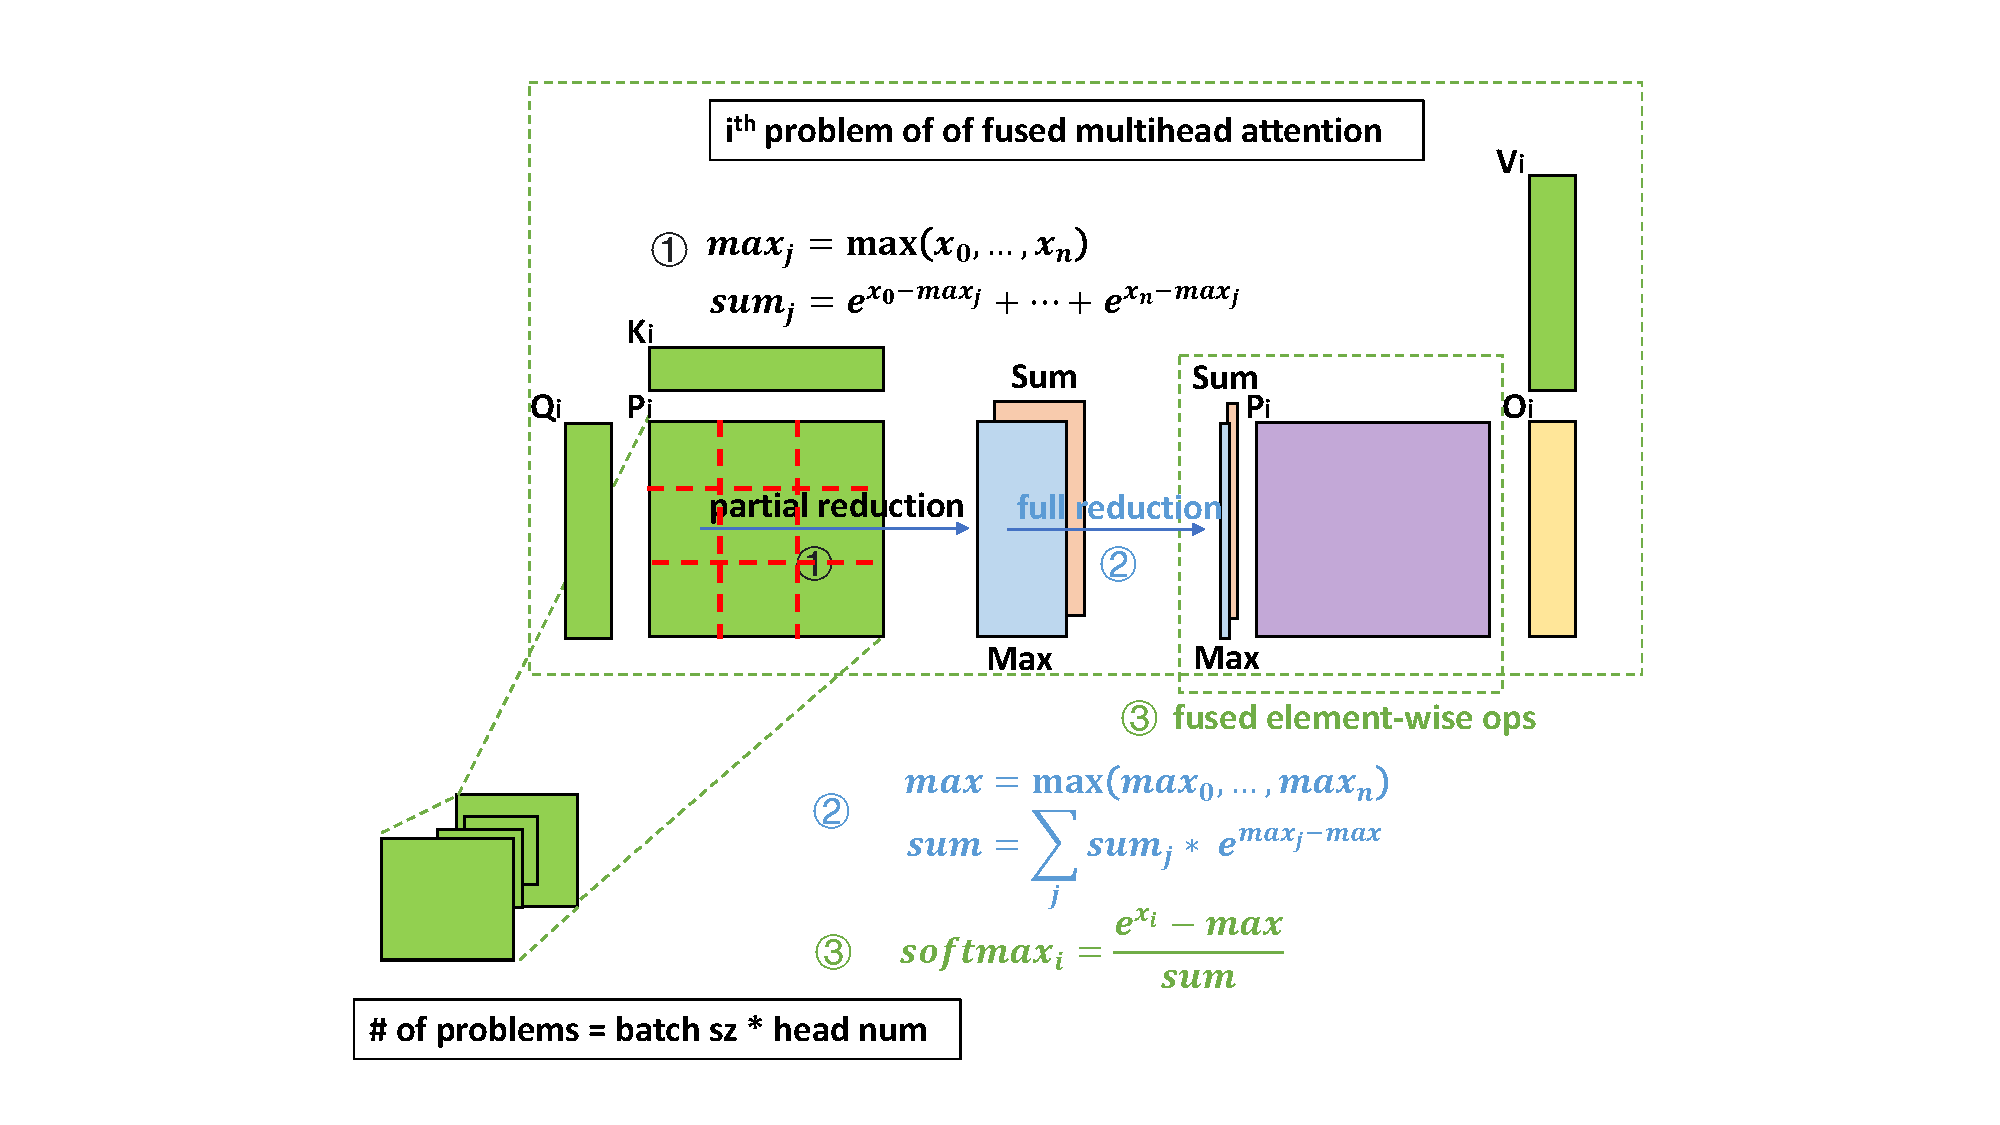
\includegraphics[width=1.\textwidth]{./images/grouped-mha.pdf}
                \caption{Grouped GEMM-based fused MHA.}
            \end{figure}  
        \end{column}
    \end{columns}    
\end{frame}